\documentclass{article}\usepackage[]{graphicx}\usepackage[]{xcolor}
% maxwidth is the original width if it is less than linewidth
% otherwise use linewidth (to make sure the graphics do not exceed the margin)
\makeatletter
\def\maxwidth{ %
  \ifdim\Gin@nat@width>\linewidth
    \linewidth
  \else
    \Gin@nat@width
  \fi
}
\makeatother

\definecolor{fgcolor}{rgb}{0.345, 0.345, 0.345}
\newcommand{\hlnum}[1]{\textcolor[rgb]{0.686,0.059,0.569}{#1}}%
\newcommand{\hlstr}[1]{\textcolor[rgb]{0.192,0.494,0.8}{#1}}%
\newcommand{\hlcom}[1]{\textcolor[rgb]{0.678,0.584,0.686}{\textit{#1}}}%
\newcommand{\hlopt}[1]{\textcolor[rgb]{0,0,0}{#1}}%
\newcommand{\hlstd}[1]{\textcolor[rgb]{0.345,0.345,0.345}{#1}}%
\newcommand{\hlkwa}[1]{\textcolor[rgb]{0.161,0.373,0.58}{\textbf{#1}}}%
\newcommand{\hlkwb}[1]{\textcolor[rgb]{0.69,0.353,0.396}{#1}}%
\newcommand{\hlkwc}[1]{\textcolor[rgb]{0.333,0.667,0.333}{#1}}%
\newcommand{\hlkwd}[1]{\textcolor[rgb]{0.737,0.353,0.396}{\textbf{#1}}}%
\let\hlipl\hlkwb

\usepackage{framed}
\makeatletter
\newenvironment{kframe}{%
 \def\at@end@of@kframe{}%
 \ifinner\ifhmode%
  \def\at@end@of@kframe{\end{minipage}}%
  \begin{minipage}{\columnwidth}%
 \fi\fi%
 \def\FrameCommand##1{\hskip\@totalleftmargin \hskip-\fboxsep
 \colorbox{shadecolor}{##1}\hskip-\fboxsep
     % There is no \\@totalrightmargin, so:
     \hskip-\linewidth \hskip-\@totalleftmargin \hskip\columnwidth}%
 \MakeFramed {\advance\hsize-\width
   \@totalleftmargin\z@ \linewidth\hsize
   \@setminipage}}%
 {\par\unskip\endMakeFramed%
 \at@end@of@kframe}
\makeatother

\definecolor{shadecolor}{rgb}{.97, .97, .97}
\definecolor{messagecolor}{rgb}{0, 0, 0}
\definecolor{warningcolor}{rgb}{1, 0, 1}
\definecolor{errorcolor}{rgb}{1, 0, 0}
\newenvironment{knitrout}{}{} % an empty environment to be redefined in TeX

\usepackage{alltt}
\usepackage[sc]{mathpazo}
\renewcommand{\sfdefault}{lmss}
\renewcommand{\ttdefault}{lmtt}
\usepackage[T1]{fontenc}
\usepackage{geometry}
\geometry{verbose,tmargin=2.5cm,bmargin=2.5cm,lmargin=2.5cm,rmargin=2.5cm}
\setcounter{secnumdepth}{2}
\setcounter{tocdepth}{2}
\usepackage[unicode=true,pdfusetitle,
 bookmarks=true,bookmarksnumbered=true,bookmarksopen=true,bookmarksopenlevel=2,
 breaklinks=false,pdfborder={0 0 1},backref=false,colorlinks=false]
 {hyperref}
\hypersetup{
 pdfstartview={XYZ null null 1}}

\makeatletter
%%%%%%%%%%%%%%%%%%%%%%%%%%%%%% User specified LaTeX commands.
\renewcommand{\textfraction}{0.05}
\renewcommand{\topfraction}{0.8}
\renewcommand{\bottomfraction}{0.8}
\renewcommand{\floatpagefraction}{0.75}

\makeatother
\IfFileExists{upquote.sty}{\usepackage{upquote}}{}
\begin{document}



\title{\title{\title{\title{\title{\title{\title{}}}}}}}



\maketitle
The results below are generated from an R script.

\begin{knitrout}
\definecolor{shadecolor}{rgb}{0.969, 0.969, 0.969}\color{fgcolor}\begin{kframe}
\begin{alltt}
\hlcom{# Librerías necesarias}
\hlkwd{library}\hlstd{(mlbench)}
\hlkwd{library}\hlstd{(dplyr)}
\hlkwd{library}\hlstd{(ggfortify)}


\hlcom{## Cargamos los datos}
\hlstd{df}\hlkwb{=}\hlstd{BostonHousing}

\hlkwd{summary}\hlstd{(df)}
\end{alltt}
\begin{verbatim}
##       crim                zn             indus       chas         nox        
##  Min.   : 0.00632   Min.   :  0.00   Min.   : 0.46   0:471   Min.   :0.3850  
##  1st Qu.: 0.08205   1st Qu.:  0.00   1st Qu.: 5.19   1: 35   1st Qu.:0.4490  
##  Median : 0.25651   Median :  0.00   Median : 9.69           Median :0.5380  
##  Mean   : 3.61352   Mean   : 11.36   Mean   :11.14           Mean   :0.5547  
##  3rd Qu.: 3.67708   3rd Qu.: 12.50   3rd Qu.:18.10           3rd Qu.:0.6240  
##  Max.   :88.97620   Max.   :100.00   Max.   :27.74           Max.   :0.8710  
##        rm             age              dis              rad              tax       
##  Min.   :3.561   Min.   :  2.90   Min.   : 1.130   Min.   : 1.000   Min.   :187.0  
##  1st Qu.:5.886   1st Qu.: 45.02   1st Qu.: 2.100   1st Qu.: 4.000   1st Qu.:279.0  
##  Median :6.208   Median : 77.50   Median : 3.207   Median : 5.000   Median :330.0  
##  Mean   :6.285   Mean   : 68.57   Mean   : 3.795   Mean   : 9.549   Mean   :408.2  
##  3rd Qu.:6.623   3rd Qu.: 94.08   3rd Qu.: 5.188   3rd Qu.:24.000   3rd Qu.:666.0  
##  Max.   :8.780   Max.   :100.00   Max.   :12.127   Max.   :24.000   Max.   :711.0  
##     ptratio            b              lstat            medv      
##  Min.   :12.60   Min.   :  0.32   Min.   : 1.73   Min.   : 5.00  
##  1st Qu.:17.40   1st Qu.:375.38   1st Qu.: 6.95   1st Qu.:17.02  
##  Median :19.05   Median :391.44   Median :11.36   Median :21.20  
##  Mean   :18.46   Mean   :356.67   Mean   :12.65   Mean   :22.53  
##  3rd Qu.:20.20   3rd Qu.:396.23   3rd Qu.:16.95   3rd Qu.:25.00  
##  Max.   :22.00   Max.   :396.90   Max.   :37.97   Max.   :50.00
\end{verbatim}
\begin{alltt}
\hlcom{# Convertimos la variable CHAS a numérica}
\hlstd{df} \hlkwb{=}
  \hlstd{df} \hlopt
  \hlkwd{mutate}\hlstd{(}\hlkwc{chas}\hlstd{=}\hlkwd{as.numeric}\hlstd{(chas))}

\hlcom{# PCA}
\hlstd{df_pca} \hlkwb{<-} \hlkwd{prcomp}\hlstd{(df[,} \hlopt{-}\hlnum{14}\hlstd{],} \hlkwc{scale}\hlstd{=} \hlnum{TRUE}\hlstd{)}
\hlkwd{summary}\hlstd{(df_pca)}
\end{alltt}
\begin{verbatim}
## Importance of components:
##                           PC1    PC2     PC3     PC4     PC5     PC6     PC7     PC8
## Standard deviation     2.4752 1.1972 1.11473 0.92605 0.91368 0.81081 0.73168 0.62936
## Proportion of Variance 0.4713 0.1103 0.09559 0.06597 0.06422 0.05057 0.04118 0.03047
## Cumulative Proportion  0.4713 0.5816 0.67713 0.74310 0.80732 0.85789 0.89907 0.92954
##                           PC9    PC10    PC11    PC12    PC13
## Standard deviation     0.5263 0.46930 0.43129 0.41146 0.25201
## Proportion of Variance 0.0213 0.01694 0.01431 0.01302 0.00489
## Cumulative Proportion  0.9508 0.96778 0.98209 0.99511 1.00000
\end{verbatim}
\begin{alltt}
\hlkwd{autoplot}\hlstd{(df_pca,}\hlkwc{data}\hlstd{=df,}\hlkwc{colour}\hlstd{=}\hlstr{'medv'}\hlstd{,}\hlkwc{loadings}\hlstd{=}\hlnum{TRUE}\hlstd{,}\hlkwc{loadings.label}\hlstd{=}\hlnum{TRUE}\hlstd{)}
\end{alltt}
\end{kframe}

{\centering 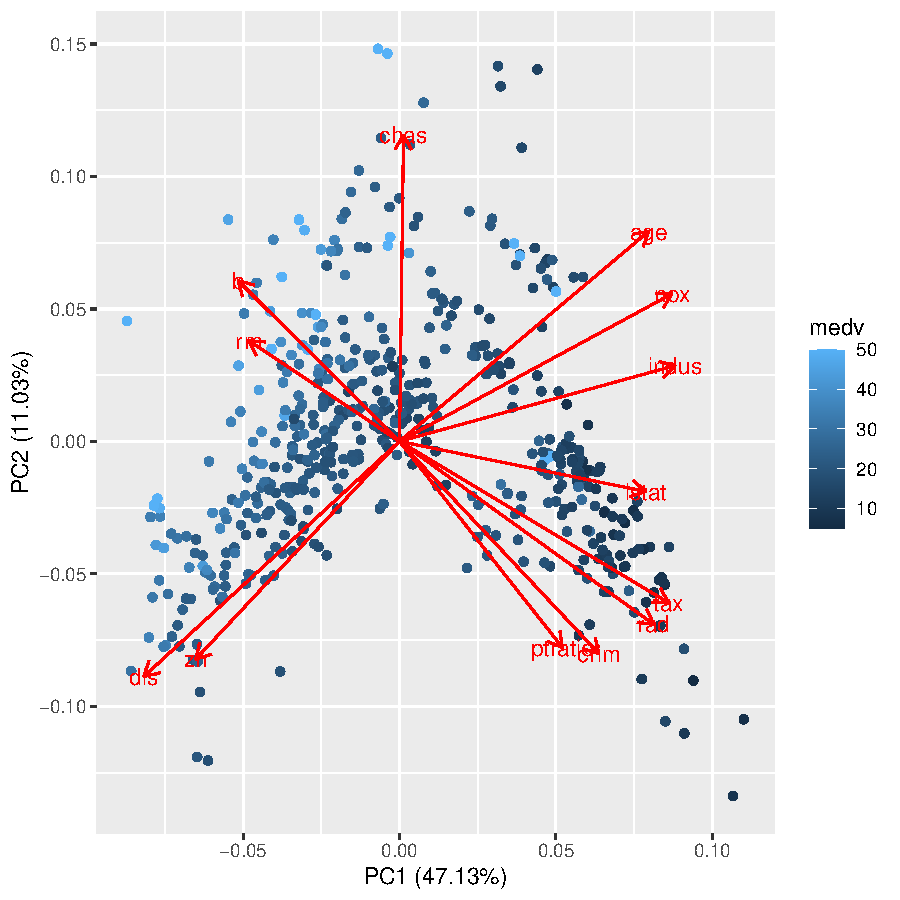
\includegraphics[width=.6\linewidth]{figure/PCA1-SOLUCION-Rnwauto-report-1} 

}


\begin{kframe}\begin{alltt}
\hlcom{# Las casas más caras parecen situarse, especialmente, en la esquina superior izquierda.}
\hlstd{df} \hlkwb{=}
  \hlstd{df} \hlopt
  \hlkwd{mutate}\hlstd{(}\hlkwc{caras}\hlstd{=}\hlkwd{as.factor}\hlstd{(}\hlkwd{ifelse}\hlstd{(medv}\hlopt{>}\hlnum{40}\hlstd{,}\hlnum{1}\hlstd{,}\hlnum{0}\hlstd{)))}

\hlkwd{autoplot}\hlstd{(df_pca,}\hlkwc{data}\hlstd{=df,}\hlkwc{colour}\hlstd{=}\hlstr{'caras'}\hlstd{,}\hlkwc{loadings}\hlstd{=}\hlnum{TRUE}\hlstd{,}\hlkwc{loadings.label}\hlstd{=}\hlnum{TRUE}\hlstd{)}
\end{alltt}
\end{kframe}

{\centering 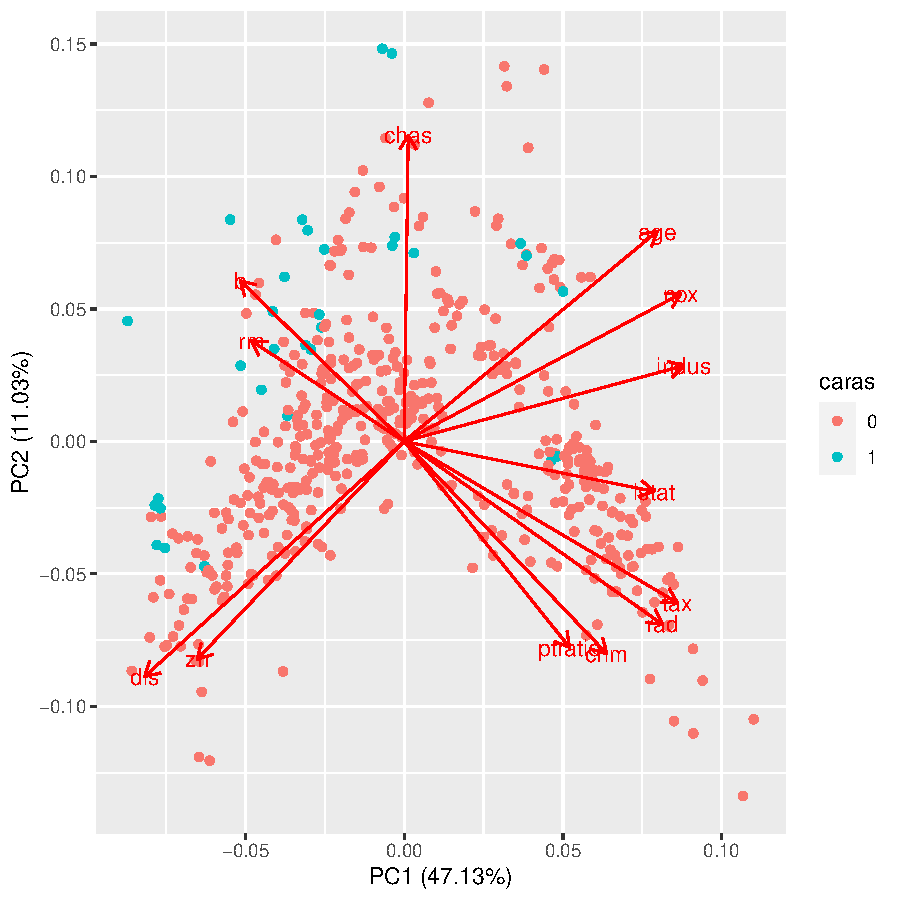
\includegraphics[width=.6\linewidth]{figure/PCA1-SOLUCION-Rnwauto-report-2} 

}


\begin{kframe}\begin{alltt}
\hlcom{# Las casas caras parecen estar asociadas a `chas`=1 y valores altos de "b" }
\hlcom{# y "rm"}

\hlcom{# Interpretación de las dos primeras componentes }
\hlstd{df_pca}\hlopt{$}\hlstd{rotation[,} \hlnum{1}\hlopt{:}\hlnum{2}\hlstd{]}
\end{alltt}
\begin{verbatim}
##                  PC1         PC2
## crim     0.250951397 -0.31525237
## zn      -0.256314541 -0.32331290
## indus    0.346672065  0.11249291
## chas     0.005042434  0.45482914
## nox      0.342852313  0.21911553
## rm      -0.189242570  0.14933154
## age      0.313670596  0.31197778
## dis     -0.321543866 -0.34907000
## rad      0.319792768 -0.27152094
## tax      0.338469147 -0.23945365
## ptratio  0.204942258 -0.30589695
## b       -0.202972612  0.23855944
## lstat    0.309759840 -0.07432203
\end{verbatim}
\begin{alltt}
\hlcom{#La primera componente principal parece tener valores elevados en las variables}
\hlcom{# `dis`, `zn`, 'b' y 'rm', frente a valores altos en todas las demas, a }
\hlcom{# excepción de la variable chas. La segunda componente principal enfrenta }
\hlcom{# observaciones con valores altos en `chas`, `age`, `nox`y `b`, frente a }
\hlcom{# observaciones con valores altos en `crim`, `zn`, `dis` y `ptratio`.}
\end{alltt}
\end{kframe}
\end{knitrout}

The R session information (including the OS info, R version and all
packages used):

\begin{knitrout}
\definecolor{shadecolor}{rgb}{0.969, 0.969, 0.969}\color{fgcolor}\begin{kframe}
\begin{alltt}
\hlkwd{sessionInfo}\hlstd{()}
\end{alltt}
\begin{verbatim}
## R version 4.3.1 (2023-06-16)
## Platform: x86_64-pc-linux-gnu (64-bit)
## Running under: Ubuntu 20.04.6 LTS
## 
## Matrix products: default
## BLAS:   /usr/lib/x86_64-linux-gnu/atlas/libblas.so.3.10.3 
## LAPACK: /usr/lib/x86_64-linux-gnu/atlas/liblapack.so.3.10.3;  LAPACK version 3.9.0
## 
## locale:
##  [1] LC_CTYPE=es_ES.UTF-8       LC_NUMERIC=C               LC_TIME=es_ES.UTF-8       
##  [4] LC_COLLATE=es_ES.UTF-8     LC_MONETARY=es_ES.UTF-8    LC_MESSAGES=es_ES.UTF-8   
##  [7] LC_PAPER=es_ES.UTF-8       LC_NAME=C                  LC_ADDRESS=C              
## [10] LC_TELEPHONE=C             LC_MEASUREMENT=es_ES.UTF-8 LC_IDENTIFICATION=C       
## 
## time zone: Europe/Madrid
## tzcode source: system (glibc)
## 
## attached base packages:
## [1] stats     graphics  grDevices utils     datasets  methods   base     
## 
## other attached packages:
##  [1] ggfortify_0.4.16 factoextra_1.0.7 mlbench_2.1-3.1  readxl_1.4.3     caret_6.0-94    
##  [6] lattice_0.21-9   ggplot2_3.4.3    rpart.plot_3.1.1 rpart_4.1.19     caTools_1.18.2  
## [11] dplyr_1.1.3      ISLR2_1.3-2     
## 
## loaded via a namespace (and not attached):
##  [1] tidyselect_1.2.0     timeDate_4022.108    farver_2.1.1         bitops_1.0-7        
##  [5] fastmap_1.1.1        pROC_1.18.4          digest_0.6.33        timechange_0.2.0    
##  [9] lifecycle_1.0.3      survival_3.5-7       magrittr_2.0.3       compiler_4.3.1      
## [13] rlang_1.1.1          tools_4.3.1          utf8_1.2.3           yaml_2.3.7          
## [17] data.table_1.14.8    knitr_1.44           labeling_0.4.3       plyr_1.8.9          
## [21] withr_2.5.1          purrr_1.0.2          nnet_7.3-19          grid_4.3.1          
## [25] stats4_4.3.1         fansi_1.0.5          e1071_1.7-13         colorspace_2.1-0    
## [29] future_1.33.0        globals_0.16.2       scales_1.2.1         iterators_1.0.14    
## [33] MASS_7.3-60          tinytex_0.47         cli_3.6.1            rmarkdown_2.25      
## [37] generics_0.1.3       rstudioapi_0.15.0    future.apply_1.11.0  reshape2_1.4.4      
## [41] tzdb_0.4.0           proxy_0.4-27         stringr_1.5.0        splines_4.3.1       
## [45] parallel_4.3.1       cellranger_1.1.0     vctrs_0.6.3          hardhat_1.3.0       
## [49] Matrix_1.6-1.1       hms_1.1.3            ggrepel_0.9.3        listenv_0.9.0       
## [53] foreach_1.5.2        tidyr_1.3.0          gower_1.0.1          recipes_1.0.8       
## [57] glue_1.6.2           parallelly_1.36.0    codetools_0.2-19     lubridate_1.9.3     
## [61] stringi_1.7.12       gtable_0.3.4         munsell_0.5.0        tibble_3.2.1        
## [65] pillar_1.9.0         htmltools_0.5.6.1    ipred_0.9-14         lava_1.7.2.1        
## [69] R6_2.5.1             evaluate_0.22        readr_2.1.4          highr_0.10          
## [73] class_7.3-22         Rcpp_1.0.11          gridExtra_2.3        nlme_3.1-163        
## [77] prodlim_2023.08.28   xfun_0.40            pkgconfig_2.0.3      ModelMetrics_1.2.2.2
\end{verbatim}
\begin{alltt}
\hlkwd{Sys.time}\hlstd{()}
\end{alltt}
\begin{verbatim}
## [1] "2023-11-01 22:05:09 CET"
\end{verbatim}
\end{kframe}
\end{knitrout}


\end{document}
